In this project it was chosen to follow an iterative development process. This was chosen because the success criteria for this project are not well defined, since the goal of picking which song to play next is a largely subjective decision.

In the iterative process, the design and implementation is done one step at a time. The development is done in iterations with a new milestone for each iteration. These milestones consist of some features which will be analysed, designed, implemented and evaluated, documenting every step in the process. Ideas for various algorithms will be tested on multiple subjects, which will be interviewed in an effort to find new possible problems or requirements, to be taken up for consideration in the following iterations.

This project being very experimental, following a linear approach could require a large amount of research which has not previously been done, for making descriptive analysis and design documents, before being able to test our theses on how to cope with the problem. Problems which arise later in the process, would then not be handled in an efficient way.

One of the problem with the incremental model compared to the linear waterfall model is that the project can lack structure, since setting milestones with clear goals can be more difficult.



We will be following these steps through each iteration:

\begin{enumerate}
  \item Gathering data from users and previous iterations
  \item An brief analysis of these data, for declaring new requirements
  \item A comprehensive design phase, researching and choosing concepts in solving these requirements
  \item An effective coding period, implementing chosen the design
  \item A test of the prototype, Unit test and among users for gathering data for future iterations
\end{enumerate}

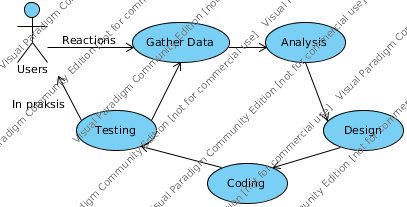
\includegraphics{Images/Developmentprocess.png}
